\providecommand{\home}{../../..}
\documentclass[\home/main.tex]{subfiles}
\usetikzlibrary[arrows,snakes,backgrounds]

\begin{document}

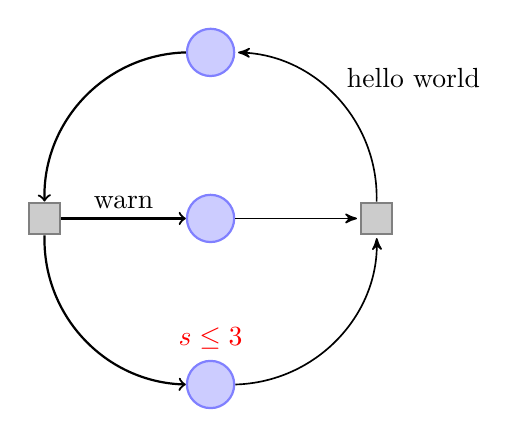
\begin{tikzpicture}[node distance = 6em, auto, thick]
    \tikzstyle{every label}=[red]

    \tikzset{
        place/.style={
                circle,draw=blue!50,fill=blue!20,thick,inner sep=0pt,minimum size=6mm
            },
        transition/.style={
                rectangle,draw=black!50,fill=black!20,thick,inner sep=0pt,minimum size=4mm
            },
        pre/.style={
                <-,shorten <=1pt,>=stealth',semithick
            },
        post/.style={
                ->,shorten >=1pt,>=stealth',semithick
            }
    }

    \node[place] (waiting) {};
    \node[place] (critical) [below of=waiting] {};
    \node[place] (semaphore) [below of=critical, label=above:$s\le3$] {};
    \node[transition] (leave critical) [right of=critical] {}
    edge [post, bend right=45]  node[auto, swap] {hello world}  (waiting)
    edge [pre]                                                  (critical)
    edge [pre, bend left=45]                                    (semaphore);

    \node[transition] (enter critical) [left of=critical] {};

    \draw [->] (enter critical) to node [] {warn} (critical);                  % edge [post] (critical)
    \draw [<-, bend left=45] (enter critical) to (waiting);     % edge [pre, bend left=45] (waiting)
    \draw [->, bend right=45] (enter critical) to (semaphore);  % edge [post, bend right=45] (semaphore);

\end{tikzpicture}
\end{document}
